%%
% This is an Overleaf template for presentations
% using the TUM Corporate Desing https://www.tum.de/cd
%
% For further details on how to use the template, take a look at our
% GitLab repository and browse through our test documents
% https://gitlab.lrz.de/latex4ei/tum-templates.
%
% The tumbeamer class is based on the beamer class.
% If you need further customization please consult the beamer class guide
% https://ctan.org/pkg/beamer.
% Additional class options are passed down to the base class.
%
% If you encounter any bugs or undesired behaviour, please raise an issue
% in our GitLab repository
% https://gitlab.lrz.de/latex4ei/tum-templates/issues
% and provide a description and minimal working example of your problem.
%%

\documentclass[
  german,            % define the document language (english, german)
  aspectratio=169,    % define the aspect ratio (169, 43)
  % handout=2on1,       % create handout with multiple slides (2on1, 4on1)
  % partpage=false,     % insert page at beginning of parts (true, false)
  % sectionpage=true,   % insert page at beginning of sections (true, false)
]{tumbeamer}


% load additional packages
\usepackage{booktabs}
\usepackage{graphicx}
\usepackage{tikz}
\usepackage{url}
\usepackage{pgfplots}
\usepackage{hyperref}
\usepackage{pmboxdraw}
\usepackage{float}
\usepackage{babel}[ngerman]
\usepackage{csquotes}[autostyle]
\usepackage[useregional]{datetime2}
\usepackage{listings}
\usepackage{xurl}
\usetikzlibrary{patterns}

% tikz
\usetikzlibrary{overlay-beamer-styles}
\usetikzlibrary{arrows.meta,backgrounds,positioning,shapes.symbols,decorations.pathreplacing,patterns,patterns.meta,tikzmark,chains,matrix,arrows,shapes.geometric}


\lstset {
    frame=single,
    tabsize=4,
    breaklines=true,
    xleftmargin=5pt,
    xrightmargin=5pt,
    basicstyle=\ttfamily\footnotesize,
    %language=[RISC-V]Assembler,
}

\hypersetup { 
  colorlinks=true,
  urlcolor=blue,
  filecolor=black,
  linkcolor=black
}

% tikz  
\usetikzlibrary{fit}

% image path
\graphicspath{ {../resources/} }

% presentation metadata
\title{Übung 05: Caches}
\subtitle{Einführung in die Rechnerarchitektur}
\author{\theAuthorName}

\institute{\theGroupName\\\theSchoolName\\\theUniversityName}
\date{18. -- \DTMdisplaydate{2024}{11}{24}{-1}}

\footline{\insertauthor~|~\insertshorttitle~|~\insertshortdate}


% macro to configure the style of the presentation
\TUMbeamersetup{
  title page = TUM tower,         % style of the title page
  part page = TUM toc,            % style of part pages
  section page = TUM toc,         % style of section pages
  content page = TUM more space,  % style of normal content pages
  tower scale = 1.0,              % scaling factor of TUM tower (if used)
  headline = TUM threeliner,      % which variation of headline to use
  footline = TUM default,         % which variation of footline to use
  % configure on which pages headlines and footlines should be printed
  headline on = {title page},
  footline on = {every page, title page=false},
}


% available frame styles for title page, part page, and section page:
% TUM default, TUM tower, TUM centered,
% TUM blue default, TUM blue tower, TUM blue centered,
% TUM shaded default, TUM shaded tower, TUM shaded centered,
% TUM flags
%
% additional frame styles for part page and section page:
% TUM toc
%
% available frame styles for content pages:
% TUM default, TUM more space
%
% available headline options:
% TUM empty, TUM oneliner, TUM twoliner, TUM threeliner, TUM logothreeliner
%
% available footline options:
% TUM empty, TUM default, TUM infoline


\begin{document}

\maketitle

\begin{frame}[c]{Mitschriften \& Infos}{}
  \begin{minipage}[t]{\textwidth}
    \begin{columns}[c]
      \begin{column}{0.8\textwidth}
        Montags: \href{\zulipMo}{\zulipMo}
      \end{column}
      \begin{column}{0.2\textwidth}
        \includegraphics[width=0.8\linewidth]{\zulipMoQrFilename}
      \end{column}
    \end{columns}
  \end{minipage}
  \rule{\textwidth}{0.4pt}
  \begin{minipage}[t]{\textwidth}
    \begin{columns}[c]
      \begin{column}{0.8\textwidth}
        Donnerstags: \href{\zulipDo}{\zulipDo}
      \end{column}
      \begin{column}{0.2\textwidth}
        \includegraphics[width=0.8\linewidth]{\zulipDoQrFilename}
      \end{column}
    \end{columns}
  \end{minipage}
  \ifdefined\myWebsite
  \rule{\textwidth}{0.4pt}
  \centering
  Website: \href{\myWebsite}{\myWebsite}
  \fi
\end{frame}

\begin{frame}[c]{}{}
  \begin{center}
    \LARGE  Keine Garantie für die Richtigkeit der Tutorfolien.

    \Large Bei Unklarheiten/Unstimmigkeiten haben VL/ZÜ-Folien recht!
  \end{center}
\end{frame}

\begin{frame}[c]{Inhaltsübersicht}{}
  \begin{columns}[c]
    \begin{column}{1\textwidth}
      \begin{itemize}
        \item Wiederholung
        \item Tutorblatt
        \begin{itemize}
          \item Calling Convention
          \item Rekursion in der Theorie
          \item Größter gemeinsamer Teiler
        \end{itemize}
      \end{itemize}
    \end{column}
  \end{columns}
\end{frame}

\begin{frame}[fragile, c]{Caches}{}
  \begin{itemize}
    \item Zugriffe auf Hauptspeicher ($\equiv$ RAM) sind \textbf{extrem} langsam. Lösung: Caches
    \item \enquote{Zwischenstation} zwischen Registern (sehr schnell, sehr klein) und Hauptspeicher (sehr langsam, sehr groß)
    \item Idee: Häufig genutzte Daten im Cache zwischenspeichern, der Rest wird bei Bedarf aus dem Hauptspeicher geholt
    \item heutzutage meist L1/L2/L3-Caches: Caches aufsteigender Größe, aber absteigender Zugriffszeit
  \end{itemize}
\end{frame}


\begin{frame}[c, fragile]{Terminologie}
  \begin{itemize}
    \item \textbf{Hit}: Datum liegt im Cache, \textbf{Miss}: Datum nicht im Cache, muss erst aus Hauptspeicher geholt werden
    \item Ziel: möglichst hohe \textbf{Hitrate} (Hits/Anfragen), d.h. häufig genutzte Daten liegen im Cache
    \item \textbf{zeitliche Lokalität}: Zugriff auf x $\rightarrow$ wschl. Zugriff auf x in Zukunft
    \item \textbf{räumliche Lokalität}: Zugriff auf x $\rightarrow$ Zugriff auf Daten in der Nähe (oft durch Cacheline abgedeckt)
    \item Verdrängungsstrategien: Random, LRU, LFU, FIFO
  \end{itemize}
\end{frame}

\begin{frame}[c, fragile]{Cachestrukturen}
  \begin{itemize}
    \item Direct Mapped Cache: direkte Abbildung Hauptspeicheradresse $\rightarrow$ Cache-Adresse (jede Cachezeile kann nur an einer bestimmten Stelle im Cache stehen)
    \item Fully Associative Cache: eine Cacheline kann an einer beliebigen Stelle im Cache stehen
    \item Set Associative Cache (Mengenassoziativer Cache): Aufteilung in sog. Sets, Set wird durch Adresse bestimmt, aber innerhalb des Sets kann die Cacheline an einer bel. Stelle stehen
    \item Tag: Identifikation der Cacheline im Set, Index: bestimmt Set im Cache, Offset: bestimmt Datum innerhalb einer Cacheline
    \item Tag, Index, Offset werden aus Adresse eines Zugriffs berechnet
    \item In jeder Cachezeile liegen mehrere Speicherzellen (deswegen Offset benötigt)
  \end{itemize}
\end{frame}

\begin{frame}[c, fragile]{Klassifikation von Misses}
  \resizebox{\textwidth}{!}{
    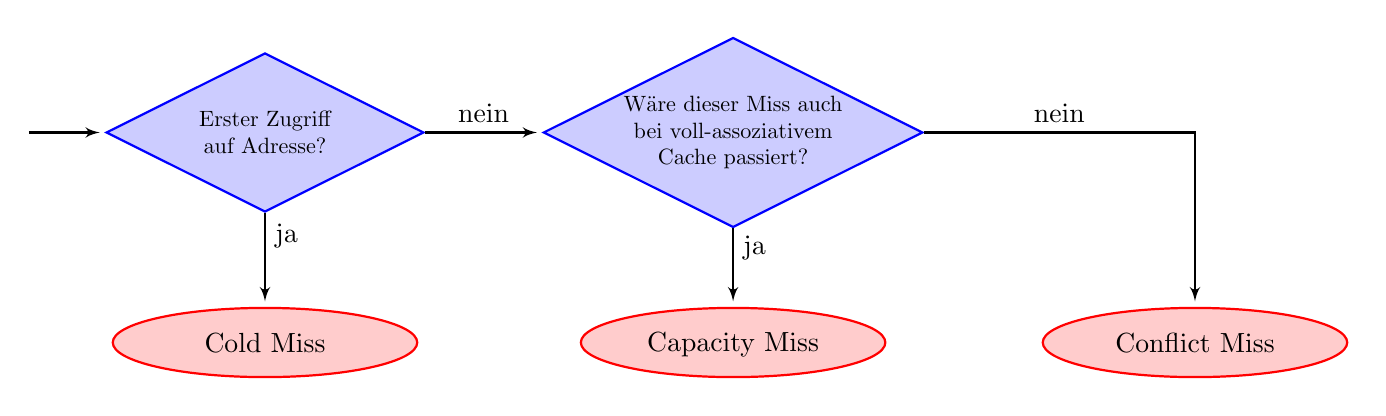
\begin{tikzpicture}
        [auto,
        ampersand replacement=\&,
        decision/.style={diamond, draw=blue, thick, fill=blue!20, text width=35mm, align=center, inner sep=1pt, scale=0.8, aspect=2},
        line/.style={draw, thick, -latex',shorten >=2pt},
        cloud/.style={draw=red, thick, ellipse,fill=red!20,
            minimum height=2.5em, text width=25mm, align=center, text depth=0pt}]
        
        \matrix [column sep=15mm,row sep=10mm]
        {
            \node [decision] (iscoldmiss) {Erster Zugriff auf Adresse?};
            \& \node [decision] (iscapmiss) {Wäre dieser Miss auch bei voll-assoziativem Cache passiert?}; \&\\
            \node [cloud] (coldmiss) {Cold Miss};
            \& \node [cloud] (capacitymiss) {Capacity Miss};
            \& \node [cloud] (conflictmiss) {Conflict Miss};\\
        };
        \begin{scope}[every path/.style=line]
            \path (iscoldmiss) + (left:30mm) -- (iscoldmiss);
            \path (iscoldmiss) -- node [near start] {ja} (coldmiss);
            \path (iscoldmiss) -- node [midway] {nein} (iscapmiss);
            \path (iscapmiss)  -- node [near start] {ja} (capacitymiss);
            \path (iscapmiss)  -| node [near start] {nein} (conflictmiss);
        \end{scope}
\end{tikzpicture}}
\vfill
\begin{center}
  \scriptsize Nach Gschoßmann et al., 2023
\end{center}
\end{frame}

\begin{frame}[c, fragile]{Ein paar Formeln$\ldots$}
  Für einen n-assoziativen Cache (jeweils n Cachezeilen in einem Set):
  \vspace{0.25cm}
  \begin{itemize}
    \item $\textrm{Anzahl Cache-Lines}=\frac{\textrm{Cachegröße}}{\textrm{Cachezeilengröße}}$
    \item $\textrm{Anzahl Cache-Sets}=\frac{\textrm{Anzahl Cache-Lines}}{\textrm{n}}$
    \item $\textrm{Anzahl Index-Bits}=\lceil\log_2(\textrm{Anzahl Cache-Sets})\rceil$
    \item $\textrm{Anzahl Offset-Bits}=\lceil\log_2(\textrm{Cachezeilengröße})\rceil$
    \item $\textrm{Anzahl Tag-Bits}= \textrm{Anzahl Adressbits} - \textrm{Anzahl Index-Bits} - \textrm{Anzahl Offset-Bits}$
  \end{itemize}
\end{frame}

\begin{frame}[c]{}{}
  \begin{center}
    \LARGE Fragen?
  \end{center}
  \vspace{0.5cm}
  \begin{center}
    \LARGE Bis zum nächsten Mal ;) \\
  \end{center}
  \vspace{1.0cm}
  \begin{center}
    \small Folien inspiriert von Niklas Ladurner
  \end{center}
\end{frame}

\end{document}